% This must be in the first 5 lines to tell arXiv to use pdfLaTeX, which is strongly recommended.
\pdfoutput=1
% In particular, the hyperref package requires pdfLaTeX in order to break URLs across lines.

\documentclass[11pt]{article}

% Remove the "review" option to generate the final version.
\usepackage[review]{EMNLP2023}
% \usepackage{EMNLP2023}

% Standard package includes
\usepackage{times}
\usepackage{latexsym}

% For proper rendering and hyphenation of words containing Latin characters (including in bib files)
\usepackage[T1]{fontenc}
% For Vietnamese characters
% \usepackage[T5]{fontenc}
% See https://www.latex-project.org/help/documentation/encguide.pdf for other character sets

% This assumes your files are encoded as UTF8
\usepackage[utf8]{inputenc}

% This is not strictly necessary and may be commented out.
% However, it will improve the layout of the manuscript,
% and will typically save some space.
\usepackage{microtype}

% This is also not strictly necessary and may be commented out.
% However, it will improve the aesthetics of text in
% the typewriter font.
\usepackage{inconsolata}

\usepackage{booktabs}
\usepackage{amssymb}
\usepackage{pifont}% http://ctan.org/pkg/pifont
\newcommand{\cmark}{\ding{51}}%
\newcommand{\xmark}{\ding{55}}%
\usepackage{graphics}


% If the title and author information does not fit in the area allocated, uncomment the following
%
%\setlength\titlebox{<dim>}
%
% and set <dim> to something 5cm or larger.

\title{All for One and One for All: A Multi-Task Framework for Various Information Extraction Tasks}

% Author information can be set in various styles:
% For several authors from the same institution:
% \author{Author 1 \and ... \and Author n \\
%         Address line \\ ... \\ Address line}
% if the names do not fit well on one line use
%         Author 1 \\ {\bf Author 2} \\ ... \\ {\bf Author n} \\
% For authors from different institutions:
% \author{Author 1 \\ Address line \\  ... \\ Address line
%         \And  ... \And
%         Author n \\ Address line \\ ... \\ Address line}
% To start a separate ``row'' of authors use \AND, as in
% \author{Author 1 \\ Address line \\  ... \\ Address line
%         \AND
%         Author 2 \\ Address line \\ ... \\ Address line \And
%         Author 3 \\ Address line \\ ... \\ Address line}

% \author{First Author \\
%   Affiliation / Address line 1 \\
%   Affiliation / Address line 2 \\
%   Affiliation / Address line 3 \\
%   \texttt{email@domain} \\\And
%   Second Author \\
%   Affiliation / Address line 1 \\
%   Affiliation / Address line 2 \\
%   Affiliation / Address line 3 \\
%   \texttt{email@domain} \\}

\author{First Author \\
  Affiliation / Address line 1 \\
  Affiliation / Address line 2 \\
  Affiliation / Address line 3 \\
  \texttt{email@domain} \\\And
  Second Author \\
  Affiliation / Address line 1 \\
  Affiliation / Address line 2 \\
  Affiliation / Address line 3 \\
  \texttt{email@domain} \\}


\begin{document}
\maketitle

\begin{abstract}

The variety of information extraction tasks and data formats make it hard to share common knowledge among those tasks.
This causes wastes to some extent and adds difficulties to build complex pipeline applications in real scenarios.
Recent studies formulate IE tasks as a triplet extraction problem.
However, such format does not support multi-span and n-ary extraction tasks, leading to weak versatility.
To this end, we reorganize IE datasets into a unified format and propose a universal framework for various IE tasks, namely Mirror.
We regard IE tasks as a multi-span cyclic graph extraction problem, and devise a non-autoregressive graph decoding algorithm to extract all spans in a single step.
This graph structure is flexible, and it supports span-only MRC, label-only classification, and label-span mixed information extraction tasks.
We manually construct a corpus containing 62 datasets for model pretraining, and experiments on 30 datasets across 8 tasks show that our model has good compatibilities and achieves SOTA performances under few-shot and zero-shot settings.
The code, model weights and data will be publicly available at GitHub.

\end{abstract}
\section{Introduction}

Information Extraction (IE) is a fundamental task in Natural Language Processing (NLP), which aims to extract structured information from unstructured text~\cite{grishman_2019}, such as Named Entity Recognition (NER), Relation Extraction (RE), Event Extraction (EE), etc.
However, each IE task is usually isolated with specific data structures and delicate models, which makes it difficult to share knowledge across tasks~\cite{uie,genie}.

In order to unify the data formats and take advantage of common features between different tasks, there are two main routes in recent studies.
The first is to utilize generative pretrained language models (PLMs) to generate the structured information directly.
\citet{uie} and \citet{tanl} structure the IE tasks as a sequence-to-sequence problem, and use generative models to predict the structured information autoregressively.
However, such methods cannot provide the exact positions of the structured information, which is important for NER and fair evaluations~\cite{devil-ee}.
Besides, the generation-based methods are usually slow, and it consumes huge resources to train on large-scale datasets~\cite{deepstruct}.
The second is to apply the extractive PLMs, which is way more faster to train and inference.
USM takes the IE tasks into a triplet prediction problems via semantic matching~\cite{usm}.
However, such method is limited in a small range of triplet-based tasks, and not suitable for multi-span and n-ary IE tasks.

\begin{figure}[t]
    \centering
    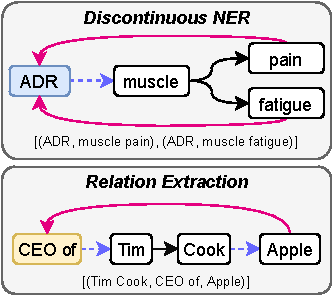
\includegraphics[width=\columnwidth]{figs/Multi-span Cyclic Graph.pdf}
    \caption{
        Multi-span cyclic graph for discontinuous NER and RE tasks (best viewed in color).
        The spans are connected by three types of edges, including \textbf{\textit{consecutive connections}}, dotted \textbf{\color[HTML]{695efb} \textit{jump connections}} and \textbf{\color[HTML]{E9087F} \textit{tail-to-head connections}}.
        \textit{ADR} in discontinuous NER denotes the entity label of Adverse Drug Reaction.
    }
    \label{fig:multi-span-cyclic-graph}
\end{figure}

\begin{table*}[t]
    \centering
    % \resizebox{\textwidth}{!}{%
        \begin{tabular}{c|ccccc|c}
        \toprule
        Model       & TANL    & UIE      & DeepStruct & InstructUIE & USM        & Mirror \\
        \midrule
        PLM         & T5-base & T5-large & GLM        & FlanT5 & RoBERTa    & DeBERTa-v3 \\
        \#Params    & 220M    & 770M     & 10B        & 11B & large 372M & large 434M \\
        \midrule
        % Single-step & {\color[HTML]{008114}\cmark}    & {\color[HTML]{008114}\cmark}   & {\color[HTML]{008114}\cmark} & {\color[HTML]{008114}\cmark} & {\color[HTML]{008114}\cmark} \\
        % NAR         & \textcolor{red}{\xmark}         & \textcolor{red}{\xmark}        & \textcolor{red}{\xmark}      & {\color[HTML]{008114}\cmark} & {\color[HTML]{008114}\cmark} \\
        Decoding    & AR                      & AR                      & AR                      & AR                      & NAR                          & NAR                          \\
        Indexing    & \textcolor{red}{\xmark} & \textcolor{red}{\xmark} & \textcolor{red}{\xmark} & \textcolor{red}{\xmark} & {\color[HTML]{008114}\cmark} & {\color[HTML]{008114}\cmark} \\
        \midrule
        Triplet     & {\color[HTML]{008114}\cmark} & {\color[HTML]{008114}\cmark} & {\color[HTML]{008114}\cmark} & {\color[HTML]{008114}\cmark} & {\color[HTML]{008114}\cmark} & {\color[HTML]{008114}\cmark} \\
        Single-span NER & {\color[HTML]{008114}\cmark} & {\color[HTML]{008114}\cmark} & {\color[HTML]{008114}\cmark} & {\color[HTML]{008114}\cmark} & {\color[HTML]{008114}\cmark} & {\color[HTML]{008114}\cmark} \\
        Multi-span  & \textcolor{red}{\xmark} & $\circ$                 & $\circ$                 & $\circ$                 & \textcolor{red}{\xmark} & {\color[HTML]{008114}\cmark} \\
        N-ary       & \textcolor{red}{\xmark} & \textcolor{red}{\xmark} & \textcolor{red}{\xmark} & \textcolor{red}{\xmark} & \textcolor{red}{\xmark} & {\color[HTML]{008114}\cmark} \\
        Cls.        & \textcolor{red}{\xmark} & \textcolor{red}{\xmark} & \textcolor{red}{\xmark} & $\circ$                 & \textcolor{red}{\xmark} & {\color[HTML]{008114}\cmark} \\
        MRC         & \textcolor{red}{\xmark} & \textcolor{red}{\xmark} & \textcolor{red}{\xmark} & \textcolor{red}{\xmark} & $\circ$                 & {\color[HTML]{008114}\cmark} \\
        \bottomrule
        \end{tabular}
    % }
    \caption{
        Comparisons with other systems.
        % Single-step represents that the model predicts results in a single step.
        \textbf{Circle} $\circ$ indicates the model supports the task theoretically, but the implementation is not available.
        \textbf{AR} denotes the auto-regressive decoding while \textbf{NAR} is the non-autoregressive decoding strategy.
        \textbf{Indexing} means whether the model could provide exact information positions.
        \textbf{Triplet} stands for ``(head, relation, tail)'' triplet extraction.
        \textbf{Single-span NER} denotes flat, and nested NER tasks with consecutive spans.
        \textbf{Multi-span} means the model supports multi-span extraction, e.g. the discontinuous named entity recognition task.
        \textbf{N-ary} denotes the ability of n-ary tuple extraction, e.g. quadruple extraction.
        \textbf{Cls.} represents the classfication and multi-choice Machine Reading Comprehension (MRC) support.
        \textbf{MRC} stands for extractive Question Answering (QA) and extractive MRC task support.
    }
    \label{tab:method_comparison}
\end{table*}

% \begin{table*}[t]
%     \centering
%     \resizebox{\textwidth}{!}{%
%         \begin{tabular}{c|ccccccc|c}
%         \toprule
%         Model & TANL & UIE & DeepStruct & InstructUIE & USM & UniEX & RexUIE & Mirror \\
%         \midrule
%         PLM & T5-base & T5-large & GLM & FlanT5 & RoBERTa & RoBERTa & DeBERTa-v3 & DeBERTa-v3 \\
%         \#Params & 220M & 770M & 10B & 11B & large 372M & large 372M & large 434M & large 434M \\
%         \midrule
%         Single-step & {\color[HTML]{008114}\cmark}    & {\color[HTML]{008114}\cmark}   & {\color[HTML]{008114}\cmark}          & {\color[HTML]{008114}\cmark}           & {\color[HTML]{008114}\cmark}   & {\color[HTML]{008114}\cmark}     & \textcolor{red}{\xmark}      & {\color[HTML]{008114}\cmark}      \\
%         Indexing & \textcolor{red}{\xmark} & \textcolor{red}{\xmark} & \textcolor{red}{\xmark} & \textcolor{red}{\xmark} & {\color[HTML]{008114}\cmark} & {\color[HTML]{008114}\cmark} & {\color[HTML]{008114}\cmark} & {\color[HTML]{008114}\cmark} \\
%         NAR         & \textcolor{red}{\xmark}    & \textcolor{red}{\xmark}   & \textcolor{red}{\xmark}          & \textcolor{red}{\xmark}           & {\color[HTML]{008114}\cmark}   & {\color[HTML]{008114}\cmark}     & {\color[HTML]{008114}\cmark}      & {\color[HTML]{008114}\cmark}      \\
%         Multi-span  & \textcolor{red}{\xmark}    & $\circ$    & $\circ$           & $\circ$            & \textcolor{red}{\xmark}   & \textcolor{red}{\xmark}     & \textcolor{red}{\xmark}      & {\color[HTML]{008114}\cmark}      \\
%         N-ary       & \textcolor{red}{\xmark}    & \textcolor{red}{\xmark}   & \textcolor{red}{\xmark}          & \textcolor{red}{\xmark}           & \textcolor{red}{\xmark}   & \textcolor{red}{\xmark}     & {\color[HTML]{008114}\cmark}      & {\color[HTML]{008114}\cmark} \\
%         \bottomrule
%         \end{tabular}
%     }
%     \caption{
%         Comparisons with other systems.
%         Single-step represents that the model predicts results in a single step.
%         Indexing means whether the model could provide exact information positions.
%         NAR denotes the non-autoregressive decoding strategy.
%         Multi-span means the model supports multi-span extraction, e.g. the discontinuous named entity recognition task.
%         N-ary denotes the ability of n-ary tuple extraction.
%         $\circ$ means the model supports the task theoretically, but the implementation is not available.
%     }
%     \label{tab:method_comparison}
% \end{table*}

To extend the universal IE system into more tasks, we propose \textit{Mirror}, a new IE framework that can be applied in multi-span extraction, n-ary extraction, machine reading comprehension (MRC) and even classification tasks.
As examplified in Figure~\ref{fig:multi-span-cyclic-graph}, we formulate IE tasks into a unified multi-slot tuple extraction problem, and transform those tuples into multi-span cyclic graphs.
This graph structure is rather flexible and scalable.
It can be applied to span-only MRC tasks, label-only classification tasks, and label-span mixed IE tasks.
Mirror takes schemas as part of the model inputs, and this benefits few-shot and zero-shot tasks naturally.

% how well did we do it
We conduct extensive experiments on 30 datasets from 8 tasks, including NER, RE, EE, Aspect-based Sentiment Analysis (ABSA), multi-span discontinuous NER, n-ary hyper RE, MRC and classfication.
To enhance the few-shot and zero-shot abilities, we manually collect 57 datasets into a whole corpus for model pretraining.
Our Mirror shows good compatibility across different tasks and datasets, and achieves competitive results on few-shot and zero-shot settings.

% contribution
Our contributions are summarized as follows:
\begin{itemize}
    \item We propose a unified schema-guided multi-slot extraction paradigm, which is capable of span-only MRC, label-only classification and label-span mixed information extraction tasks.
    \item We propose Mirror, a universal non-autoregressive framework that transforms multiple tasks into a multi-span cyclic graph.
    \item We conduct extensive experiments on 30 datasets from 8 tasks, and the results show that our model achieves competitive results on single-tasks, and outperforms previous SOTA systems on few-shot and zero-shot settings.
\end{itemize}

\section{Related Work}

\subsection{Multi-task Information Extraction}

Multi-task IE is a popular research topic in recent years.
The main idea is to use a single model to perform multiple IE tasks.
IE tasks could be formulated as different graph structures.
\citet{w2ner} formulate flat, nested, and discontinuous NER tasks as a graph with next-neighboring and tail-to-head connections.
Maximal cliques also have been used to flat \& discontinuous NER tasks \cite{mac-discontinuous-ner} and trigger-available \& trigger-free event extractions \cite{ptpcg}.
DyGIE++ takes NER, RE and EE tasks as span graphs, and apply iterative propagation to enhance spans' contextual representations \cite{dygiepp}.
OneIE uses the similar graph structures with global constraint features \cite{oneie}.

In addition to explicit graph-based multi-task IE systems, generative language models are also been widely used.
\citet{bart-ner} and \citet{bart-absa} add special index tokens into BART \cite{bart} vocabulary to help perform various NER and ABSA tasks and obtain explicit span positions.
TANL \cite{tanl} apply T5 \cite{t5} to generate texts with special enclosures as the predicted information.
GenIE \cite{genie} and DeepStruct \cite{deepstruct} share a similar idea to generate subject-relation-object triplets, and DeepStruct extends the model size to 10B with GLM as the backbone \cite{glm}.


\begin{figure*}[t]
    \centering
    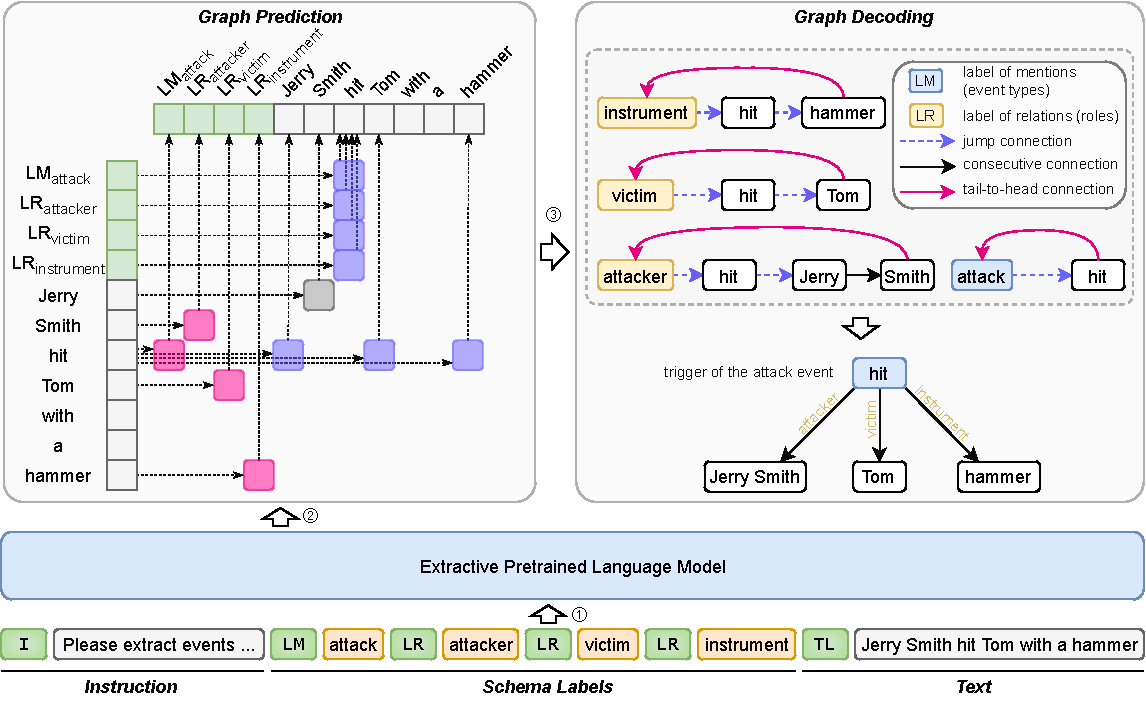
\includegraphics[width=\textwidth]{figs/Model Framework.pdf}
    \caption{Model framework (best viewed in color).}
    \label{fig:model-framework}
\end{figure*}

\subsection{Schema-guided Information Extraction}

In schema-guided IE systems, schemas are input as an guidance signal to help the model extracting target information.
UIE \cite{uie} categorize IE tasks into span spotting and asscociating elementary tasks and devise a linearized query language.
\citet{lasuie} introduces the hyper relation extraction task to represent complex IE tasks like EE, and utilize external parsing tools to enhance the text representations.
InstructUIE \cite{instructuie} formulates schemas into instructions and uses FlanT5-11B \cite{flan-t5} to performing multi-task instruction tuning.

While the above methods use flexible generative language models, they cannot predict exact positions, which brings ambiguity when evaluating.
Besides, large generative language models are usually slow to train and inference, and requires tons of computing resources.
USM \cite{usm} and UniEX \cite{uniex} utilize BERT-family models to extract triplets non-autoregressively.
USM regards IE tasks into a unified schema matching task and use a label-text matching model to extract triplets.
UniEX inherits the idea and uses a triaffine module to predict hyper-dimensional links.
Beyond triplets extraction, RexUIE \cite{rexuie} perform to extract n-ary tuples step-by-step.
Although RexUIE supports n-ary extraction, it sacrifices the efficiency and requires more time when predicting results (one slot per step).

\section{Mirror}


\begin{figure*}[t]
    \centering
    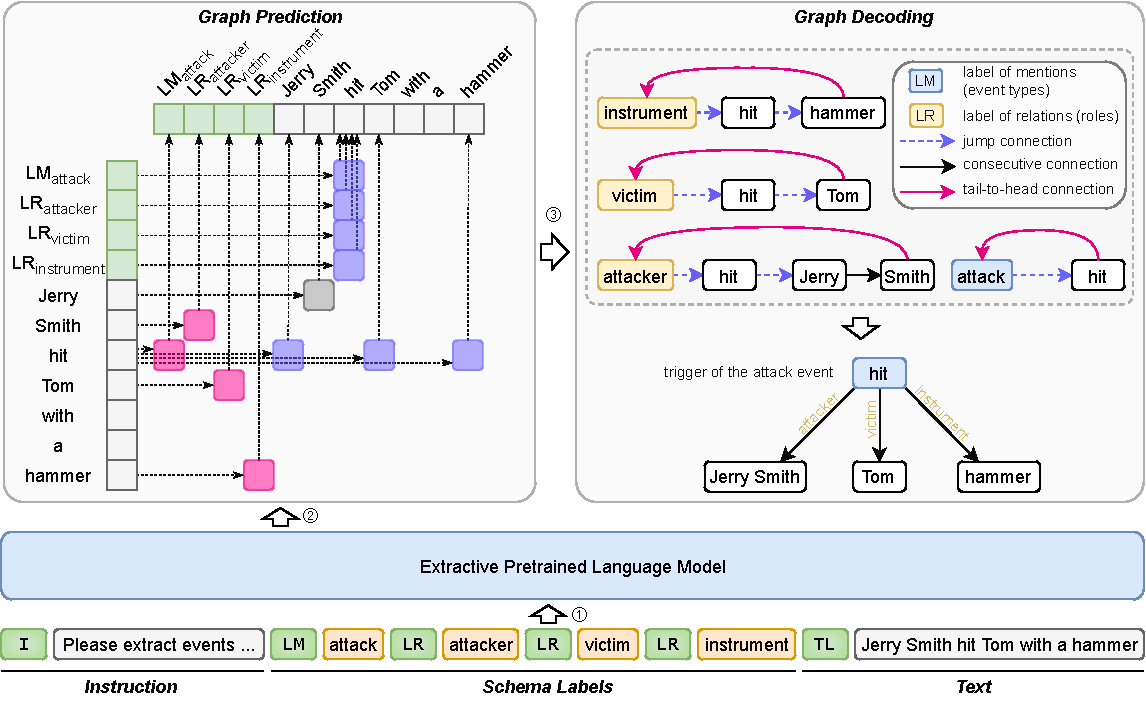
\includegraphics[width=\textwidth]{figs/Model Framework.pdf}
    \caption{Model framework (best viewed in color).}
    \label{fig:model-framework}
\end{figure*}

In this section, we introduce the Mirror framework.
We first address the unified data input format to the model, then introduce the unified task formulation and the model structure.

\subsection{Unified Data Interface}

To make the model able to handle different IE tasks, we propose a unified data interface for the model input.
As shown in Figure~\ref{fig:unified-data-interface}, there are three parts: the \textit{instruction}, the \textit{schema labels}, and the \textit{text}.
The instruction is composed of a leading token \verb|[I]| and a natural language sentence.
The leading token indicates the instruction part while the sentence tells the model what it should do.
For example, the instruction of NER could be \textit{Please identify any possible entities in the given text and label them with the following types}.
The instruction is the question in Machine Reading Comprehension (MRC) and Question Answering (QA) datasets.

The schema labels are task ontologies that used for schema-guided extraction.
This part is consists of special token labels (\verb|[LM]|, \verb|[LR]| and \verb|LC|) and corresponding label texts.
Among the special tokens, \verb|[LM]| denotes the label of mentions (or event types), \verb|[LR]| denotes the label of relations (or argument roles), and \verb|[LC]| denotes the label of classes.
\verb|[LC]| token is designed for classification tasks when pretraining.

The text part is the input text that the model should extract information from.
It is composed of a leading token (\verb|[TL]| or \verb|[TP]|) and a natural language sentence.
If the leading token is \verb|[TL]|, the model should link labels from schema labels to spans in the text.
While the \verb|[TP]| token indicates the target spans are only in the text, and the model should extract information from the text without schema labels.
The \verb|[TP]| label is used in the pretraining stage to make the model able to extract information in MRC tasks without schema.
In classification tasks when pretraining, the model should not extract anything from the text part.
So we add a special background area with a leading token \verb|[B]| to distinguish from extractive texts.

With the above three parts, we can formulate classification, extractive MRC (and extractive QA), multi-choice MRC, and IE tasks into a unified data interface, and the model can be trained in a unified way even the model is not based on generative language models.
For the robust model training, we manually collect 57 datasets across 5 tasks to make a corpus for model pretraining.
To balance the number of examples in each task, we randomly sample instances for each dataset.
If the number of instances in a dataset is less than the sampling value, we keep the original dataset unchanged and do not perform over sampling.
For NER, RE and EE tasks, we manually design a set of instructions, and randomly pick one of them for each sample.
The number of instructions for each IE task is listed in Table~\ref{tab:pretrain-dataset-statistics}.
For more detailed statistics on each dataset, please refer to Appendix~\ref{sec:appendix_data}.

\begin{table}[t]
    \centering
    \resizebox{\columnwidth}{!}{
    \begin{tabular}{lrrrr}
        \toprule
        Task & \#Dataset & \#Samples/Dataset & \#Instruction & \#Instance \\
        \midrule
        NER & 15 & 20,000 & 42 & 171,609 \\
        Cls$^{\clubsuit}$ & 27 & 5,000 & 54,070 & 134,758 \\
        RE & 9 & 20,000 & 9 & 123,876 \\
        MRC$^{\heartsuit}$ & 5 & 30,000 & 75,200 & 85,658 \\
        EE & 1 & All & 40 & 2,898 \\
        \midrule
        Total & 57 & - & - & 518,799 \\
        \bottomrule
    \end{tabular}
    }
    \caption{
        Pretraining dataset statistics.
        $^{\clubsuit}$ Classification tasks contain multi-choice MRC datasets.
        $^{\heartsuit}$ MRC stands for both extractive QA and extractive MRC datasets.
    }
    \label{tab:pretrain-dataset-statistics}
\end{table}

\subsection{Multi-slot Tuple and Multi-span Cyclic Graph}

We formulate IE tasks as a unified multi-slot tuple extraction problem.
As exemplified in Figure~\ref{fig:unified-data-interface}, in the RE task, the model is expected to extract a 3-slot tuple like \texttt{(relation, head entity, tail entity)}.
Here, the tuple is \texttt{(LR$_{\text{friend of}}$, Jerry Smith, Tom)}.
The length of tuple slots could vary across tasks, so Mirror is capable of n-ary extraction problems.

As shown in Figure~\ref{fig:multi-span-cyclic-graph} and the top right of Figure~\ref{fig:model-framework}, we formulate multi-slot tuples into a unified multi-span cyclic graph, and regard labels as the leading tokens in schema labels.
There are three types of connections in the graph: the \textbf{\textit{consecutive}} connection, the \textbf{\color[HTML]{695efb} \textit{jump}} connection, and the \textbf{\color[HTML]{E9087F}\textit{tail-to-head}} connection.
The \textbf{\textit{consecutive}} connection is adopted to \textbf{spans in the same entity}.
For an entity that has multiple tokens, the consecutive connection connects from the first token to the last token.
As shown in Figure~\ref{fig:model-framework}, ``Jerry'' connects to ``Smith''.
If there is only one token in an entity, the consecutive connection is not used.
For example, entities in ``muscle pain and fatigue'' contains two entities ``muscle pain'' and ``muscle fatigue''.
The consecutive connection is used to connect from ``muscle'' to ``pain'', and ``muscle'' to ``fatigue''.
The \textbf{\color[HTML]{695efb} \textit{jump}} connection connects \textbf{different slots} in a tuple.
Schema labels and spans from texts are in different slots, so they are connected in jump connections.
In addition, the head entity and the tail entity of a relation triplet are in different slots, so they are also connected in jump connections.
The \textbf{\color[HTML]{E9087F}\textit{tail-to-head}} connection helps \textbf{locate the start \& end boundaries}, and forms a cycle in the graph.
It connects from the last token of the last slot to the first token of the first slot in a tuple.

In practice, we convert the answer of each slot into span positions.
For schema labels, we use the position of leading tags instead of label texts.
For text spans like entities, the position is a one-digit number if there is only one character, otherwise the start and end positions are listed.
For example, the 3-slot relation tuple \texttt{(LR$_{\text{friend of}}$, Jerry Smith, Tom)} will be converted into (9 {\color[HTML]{695efb} $\vdots$} 16 $\to$ 17 {\color[HTML]{695efb} $\vdots$} 22), where $\vdots$ denotes the jump connection, $\to$ stands for the consecutive connection, 9 is the position of \texttt{LR$_{\text{friend of}}$}, 16 and 17 express \textit{Jerry Smith}, and 22 is the position of \textit{Tom}.
There is also a tail-to-head connection from 22 to 9.
The corresponding graph decoding algorithm is shown in Algorithm~\ref{alg:mcg-decoding}.
During inference, we first find the forward chain (9,16,17,22), and then verify the chain with tail-to-head connection (22$\to$9).
After that, the multi-slot tuple is revealed with jump connections(9$\vdots$16) and (17$\vdots$22).

\begin{algorithm}[t]
    \renewcommand{\algorithmicrequire}{\textbf{Input:}}
    \renewcommand{\algorithmicensure}{\textbf{Output:}}
    \caption{\textsc{Multi-span Cyclic Graph Decoding}}
    \label{alg:mcg-decoding}
    \begin{algorithmic}[1]
        \Require Adjacency matrix $\mathcal{A}$
        \Ensure A set of multi-slot tuples $\mathcal{T}$
        \State $\mathcal{T} \gets \{\}$
        \State $\tilde{\mathcal{A}} \gets \mathcal{A}^{c} | \mathcal{A}^{j}$ \Comment{merge consecutive and jump connections}
        \State Find forward chains $\mathcal{C}$ from $\tilde{\mathcal{A}}$
        \For {$c \in \mathcal{C}$}
            \Comment{find legal paths with tail-to-head connections}
            \If{$c$ meets the need in $\mathcal{A}^{t}$}
                \State split $c$ into a tuple $t$ via $\mathcal{A}^j$
                \State $\mathcal{T} \gets \mathcal{T} \cup t$
            \EndIf
        \EndFor
        \State \Return $\mathcal{T}$
    \end{algorithmic}
\end{algorithm}


\subsection{Model Structure}

With the unified data interface and the multi-span cyclic graph, we propose a unified model structure for IE tasks.
For each token $x_i$ from the inputs, Mirror transforms it into a vector $h_i \in \mathbb{R}^{d_h}$ via a BERT-style extractive pretrained language model (PLM).
Similar to \citet{ner-as-dp}, we use biaffine attention to obtain the adjacency matrix $\mathcal{A}$ of the multi-span cyclic graph.
Mirror calculates the linking probability $p_{ij}^{k}, k \in \{\text{consecutive}, \text{jump}, \text{tail-to-head}\}$ between $x_i$ and $x_j$.
The final $\mathcal{A}$ is obtained via thresholding ($\mathcal{A}_{ij}^{k}=1$ if $p_{ij}^{k} > 0.5$ else 0).
\begin{equation}
    \label{eqn:sim_calc}
    \begin{gathered}
    \tilde{h_i} = \text{FFNN}_{s}\left(h_i\right), \quad \tilde{h_j} = \text{FFNN}_{e}\left(h_j\right) \\
    p_{ij}^{k} = \text{sigmoid}\left(\tilde{h_i}^{\top} U \tilde{h_j} / \sqrt{d_h}\right)
    \end{gathered} \\
\end{equation}
% \begin{equation}
%     \label{eqn:adjacent}
%     \mathcal{A}_{i,j}^{k} = \begin{cases}
%         1 & p_{ij} > \gamma \\
%         0 & \text{otherwise}
%     \end{cases}
% \end{equation}
where $\tilde{h_i},\tilde{h_j} \in \mathbb{R}^{d_b}$.
$U \in \mathbb{R}^{d_b \times 3 \times d_b}$ is trainable parameter, and 3 denotes consecutive, jump and tail-to-head connections.
$\text{FFNN}$ is the feed forward neural network with rotary positional embedding as introduced in \citet{roformer}.
The FFNN is composed of linear transformation, GELU activation function~\cite{gelu} and dropout~\cite{dropout}.

During training, we adopt the imbalance-class multi-label categorical cross entropy~\cite{global_pointer} as the loss function.

\begin{equation}
    \label{eqn:loss}
    \mathcal{L}(i,j) = \log \left(1 + \sum_{\Omega_{\text{neg}}} e^{p_{ij}^{k}}\right) + \log \left(1 + \sum_{\Omega_{\text{pos}}} e^{-p_{ij}^{k}}\right)
\end{equation}
where $\Omega_{\text{neg}}$ stands for negative samples ($\mathcal{A}_{ij}^{k}=0$), and $\Omega_{\text{pos}}$ denotes positive samples ($\mathcal{A}_{ij}^{k}=1$).

\section{Experiments}

\subsection{Experiment Setup}

\subsection{Datasets}

\subsection{Main Results}


\begin{table*}[t]
  \resizebox{\textwidth}{!}{%
  \begin{tabular}{c|c|rrrrrrrr}
    \toprule
  Task &
    Datasets &
    \multicolumn{1}{c}{TANL} &
    \multicolumn{1}{c}{UIE} &
    \multicolumn{1}{c}{DeepStruct} &
    \multicolumn{1}{c}{InstructUIE} &
    \multicolumn{1}{c}{USM} &
    \multicolumn{1}{c}{UniEX} &
    \multicolumn{1}{c}{RexUIE} &
    \multicolumn{1}{c}{Mirror} \\
    \midrule
  \multirow{3}{*}{NER}   & ACE04     & -     & 86.89 & -    & -     & 87.62 & 87.12 & 87.25 & 87.63 \\
                         & ACE05     & 84.90 & 85.78 & 86.9 & 86.66 & 87.14 & 87.02 & 87.23 & 86.81 \\
                         & CoNLL03   & 91.70 & 92.99 & 93   & 92.94 & 93.16 & 92.65 & 93.67 & 92.83 \\
  \midrule
  \multirow{4}{*}{RE}    & ACE05     & 63.70 & 66.06 & 66.8 & -     & 67.88 & 66.06 & 64.87 & 66.70 \\
                         & CoNLL04   & 71.40 & 75.00 & 78.3 & 78.48 & 78.84 & 73.40 & 78.39 & 71.48 \\
                         & NYT       & -     & 93.54 & 93.3 & 90.47 & 94.07 & -     & 94.55 & 91.66 \\
                         & SciERC    & -     & 36.53 & -    & 45.15 & 37.36 & 38.00 & 38.37 & 36.08 \\
    \midrule
  \multirow{4}{*}{Event} & ACE05-Tgg & 68.40 & 73.36 & 69.8 & 77.13 & 72.41 & 74.08 & 75.17 & 69.95 \\
                         & ACE05-Arg & 47.60 & 54.79 & 56.2 & 72.94 & 55.83 & 53.92 & 59.15 & 48.12 \\
                         & CASIE-Tgg & -     & 69.33 & -    & 67.80 & 71.73 & 71.46 & 73.01 & 69.19 \\
                         & CASIE-Arg & -     & 61.30 & -    & 63.53 & 63.26 & 62.91 & 63.87 & 55.09 \\
  \midrule
  \multirow{4}{*}{ABSA}  & 14-res    & -     & 74.52 & -    & -     & 77.26 & 74.77 & 77.46 & 77.20 \\
                         & 14-lap    & -     & 63.88 & -    & -     & 65.51 & 65.23 & 66.41 & 62.84 \\
                         & 15-res    & -     & 67.15 & -    & -     & 69.86 & 68.58 & 70.84 & 68.82 \\
                         & 16-res    & -     & 75.07 & -    & -     & 78.25 & 76.02 & 77.20 & 75.53 \\
  \bottomrule
  \end{tabular}%
  }
  \caption{Main results.}
  \label{tab:main-results}
\end{table*}

\begin{table}[]
  % \resizebox{\columnwidth}{!}{%
  \centering
  \begin{tabular}{lrrr}
    \toprule
    & \multicolumn{1}{c}{P} & \multicolumn{1}{c}{R} & \multicolumn{1}{c}{F1} \\
    \midrule
    \multicolumn{4}{l}{\textit{Discontinuous NER: CADEC}}                           \\
    BART-NER & 70.08                 & \underline{ 71.21}           & 70.64                  \\
    W2NER    & \underline{ 74.09}           & \textbf{72.35}        & \textbf{73.21}         \\
    Mirror   & \textbf{74.83}        & 67.88                 & \underline{ 71.19}            \\
    \midrule
    \multicolumn{4}{l}{\textit{N-ary Tuples: HyperRED}}                             \\
    CubeRE   & 66.39                 & 67.12                 & 66.75                  \\
    RexUIE   & \multicolumn{1}{l}{-} & \multicolumn{1}{l}{-} & \textbf{75.20}         \\
    Mirror   & 70.88                 & 64.05                 & \underline{ 67.29} \\
    \bottomrule
  \end{tabular}%
  % }
  \caption{
    Results on multi-span and n-ary inforamtion extraction tasks.
    The best results are in \textbf{bold}, and the second best results are \underline{underlined}.
  }
  \label{tab:multi-span-n-ary-results}
\end{table}

\subsection{Few-shot Results}

\begin{table}[t]
    \centering
    \resizebox{\columnwidth}{!}{%
    \begin{tabular}{l|l|rrr|r}
    \toprule
     &
      Model &
      1-shot &
      5-shot &
      10-shot &
      \multicolumn{1}{l}{Avg.} \\
    \midrule
    \multirow{4}{*}{\shortstack{NER\\ CoNLL03}}         & UIE & 57.53 & 75.32 & 79.12 & 70.66 \\
     &
      USM &
      71.11 &
      \underline{ 83.25} &
      \underline{ 84.58} &
      79.65 \\
     &
      RexUIE &
      \textbf{86.57} &
      \textbf{89.63} &
      \textbf{90.82} &
      \textbf{89.07} \\
     &
      Mirror &
      \underline{ 77.50} &
      82.73 &
      84.48 &
      \underline{ 81.57} \\
    \midrule
    \multirow{4}{*}{\shortstack{RE\\ CoNLL04}} &
      UIE &
      34.88 &
      51.64 &
      58.98 &
      48.50 \\
     &
      USM &
      \underline{ 36.17} &
      \underline{ 53.20} &
      \underline{ 60.99} &
      \underline{ 50.12} \\
     &
      RexUIE &
      \textbf{43.80} &
      \textbf{54.90} &
      \textbf{61.68} &
      \textbf{53.46} \\
     &
      Mirror &
      34.66 &
      52.23 &
      58.68 &
      48.52 \\
      
    \midrule
    \multirow{4}{*}{\shortstack{Event Trigger\\ ACE05}} & UIE & 42.37 & 53.07 & 54.35 & 49.93 \\
     &
      USM &
      40.86 &
      55.61 &
      58.79 &
      51.75 \\
     &
      RexUIE &
      \textbf{56.95} &
      64.12 &
      \textbf{65.41} &
      \textbf{62.16} \\
     &
      Mirror &
      \underline{ 49.50} &
      \underline{ \textbf{65.61}} &
      \underline{ 60.68} &
      \underline{ 58.60} \\
      
    \midrule
    \multirow{4}{*}{\shortstack{Event Arg\\ ACE05}}     & UIE & 14.56 & 31.20 & 35.19 & 26.98 \\
     &
      USM &
      19.01 &
      36.69 &
      \underline{ 42.48} &
      32.73 \\
     &
      RexUIE &
      \textbf{30.43} &
      \underline{ 41.04} &
      \textbf{45.14} &
      \textbf{38.87} \\
     &
      Mirror &
      \underline{ 23.46} &
      \textbf{48.32} &
      41.90 &
      \underline{ 37.89} \\
      
    \midrule
    \multirow{4}{*}{\shortstack{ ABSA\\ 16res}} &
      UIE &
      23.04 &
      42.67 &
      53.28 &
      39.66 \\
     &
      USM &
      30.81 &
      \underline{ 52.06} &
      58.29 &
      47.05 \\
     &
      RexUIE &
      \underline{ 37.70} &
      49.84 &
      \underline{ 60.56} &
      \underline{ 49.37} \\
     &
      Mirror &
      \textbf{67.06} &
      \textbf{73.51} &
      \textbf{68.70} &
      \textbf{69.76} \\
    \bottomrule
    \end{tabular}%
    }
    \caption{
        Few-shot results.
        The best results are in \textbf{bold}, and the second best results are \underline{underlined}.
    }
    \label{tab:few_shot}
\end{table}

\subsection{Zero-shot Results}

\begin{table*}[t]
    % \resizebox{\textwidth}{!}{%
    \centering
    \begin{tabular}{lrrrrrrrr}
        \toprule
    Model &
      \multicolumn{1}{c}{Movie} &
      \multicolumn{1}{c}{Restaurant} &
      \multicolumn{1}{c}{AI} &
      \multicolumn{1}{c}{Literature} &
      \multicolumn{1}{c}{Music} &
      \multicolumn{1}{c}{Politics} &
      \multicolumn{1}{c}{Science} &
      \multicolumn{1}{c}{Avg.} \\
      \midrule
    Davinci          & 0.84           & 2.94           & 2.97           & 9.87           & 13.83          & 18.42          & 10.04          & 8.42           \\
    ChatGPT          & \underline{ 41.00}    & \textbf{37.76} & \textbf{54.40} & \underline{ 54.07}    & \textbf{61.24} & \underline{ 59.12}    & \textbf{63.00} & \textbf{52.94} \\
    USM              & 37.73          & 14.73          & 28.18          & \textbf{56.00} & 44.93          & 36.10          & 44.09          & 37.39          \\
    InstructUIE      & \textbf{63.00} & \underline{ 20.99}    & 49.00          & 47.21          & 53.61          & 48.15          & 49.30          & 47.32          \\
    Mirror & 40.96          & 20.02          & \underline{ 51.13}    & 44.80          & \underline{ 60.63}    & \textbf{61.19} & \underline{ 53.65}    & \underline{ 47.48}    \\
    \midrule
    Upper Bound      & 85.94          & 83.30          & 65.72          & 67.93          & 78.25          & 75.92          & 70.96          & 75.43 \\
    \bottomrule
    \end{tabular}%
    % }
    \caption{
        Zero-shot NER results.
        The best results are in \textbf{bold}, and the second best results are \underline{underlined}.
        The upper bound is the Mirror performance where these zero-shot NER training sets are included in the pretraining phase.
    }
    \label{tab:zero_shot_ner}
\end{table*}


\subsection{Analysis on Training Strategies}

\begin{table*}[t]
  \resizebox{\textwidth}{!}{%
    \begin{tabular}{ll|rrrrrr}
      \toprule
    Dataset & Training & \shortstack{NER\\ CoNLL03} & \shortstack{RE \\ CoNLL04} & \shortstack{Event Trigger\\ ACE05} & \shortstack{Event Arg\\ ACE05} & \shortstack{ ABSA\\ 16res} & Avg.  \\
    \midrule
    \multirow{2}{*}{Included in PT} & Multi-task FT  &             &             &               &               &            &       \\
                                      & Single-task FT & 92.83       & 71.48       & 69.95         & 48.12         & 75.53      & 71.58 \\
    \multirow{2}{*}{Excluded in PT} & Multi-task FT  & 91.84       & 72.39       & 68.24         & 47.73         & 75.31      & 71.10 \\
                                      & Single-task FT & 92.45       & 73.70       & 71.01         & 52.57         & 75.55      & 73.06 \\
    \bottomrule
    \end{tabular}%
  }
  \caption{Analysis on training strategy.}
  \label{tab:training-strategy}
\end{table*}

\subsection{Ablation Study}

\begin{table*}[t]
  % \resizebox{\columnwidth}{!}{%
  \begin{tabular}{l|rrrrr|r}
    \toprule
                             & \shortstack{NER\\ CoNLL03} & \shortstack{RE \\ CoNLL04} & \shortstack{Event Trigger\\ ACE05} & \shortstack{Event Arg\\ ACE05} & \shortstack{ ABSA\\ 16res} & Avg. \\
    \midrule
  Mirror                     &             &             &               &               &            &      \\
  - Pretrain                 &             &             &               &               &            &      \\
  - Pretrain \& Instruction &             &             &               &               &            &     \\
  \bottomrule
  \end{tabular}%
  % }
  \caption{Ablation study.}
  \label{tab:ablation-study}
\end{table*}

\input{src/conclusion}
\section*{Limitations}

Content input length and model compatibility.
Multi-turn result modification.
Laborious data cleaning and format unification.


\section*{Ethics Statement}

All datasets are publicly available without further annotation.
We believe there are no ethical issues in this paper.

% \section*{Acknowledgements}

This workd was supported by ...


% Entries for the entire Anthology, followed by custom entries
\bibliography{anthology,custom}
\bibliographystyle{acl_natbib}

\appendix
\section{Dataset Statistics}
\label{sec:appendix_data}


This is a section in the appendix.

\end{document}
